
% header %{{{1

\documentclass[tikz, border=1mm]{standalone}

\usepackage{amsmath}

\usetikzlibrary{calc,angles,quotes}

% document %{{{1

% opening %{{{2

\begin{document}
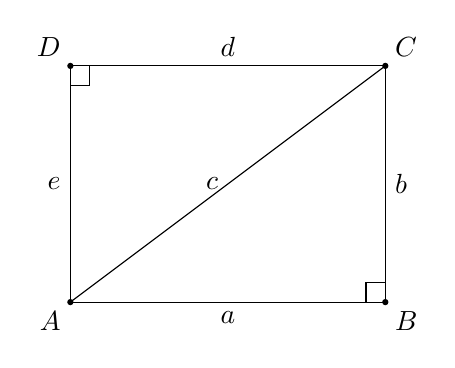
\begin{tikzpicture}[scale=1.0]

% coordinate %{{{2

	\coordinate (A) at (0,0);
	\coordinate (B) at (4,0);
	\coordinate (C) at (4,3);
	\coordinate (D) at (0,3);

% vertices %{{{2

	\fill (A) circle (0.4mm);
	\fill (B) circle (0.4mm);
	\fill (C) circle (0.4mm);
	\fill (D) circle (0.4mm);

% surrounding rectangle %{{{2

	\draw (0,0) rectangle (4,3);

% remaining side of triangle %{{{2

	\draw (A) -- (C);

% vertices labels %{{{2

	\node[below left] at (A) {$A$};
	\node[below right] at (B) {$B$};
	\node[above right] at (C) {$C$};
	\node[above left] at (D) {$D$};

% segments labels %{{{2

	\node[below] at ($(A)!0.5!(B)$) {$a$};
	\node[right] at ($(B)!0.5!(C)$) {$b$};
	\node[left] at ($(A)!0.5!(C)$) {$c$};
	\node[above] at ($(C)!0.5!(D)$) {$d$};
	\node[left] at ($(A)!0.5!(D)$) {$e$};

% right angles marks %{{{2

	\pic [draw, angle radius=7pt, angle eccentricity=1]
	{right angle = C--B--A};
	\pic [draw, angle radius=7pt, angle eccentricity=1]
	{right angle = C--D--A};

\end{tikzpicture}
\end{document}
